\documentclass[conference]{IEEEtran}
\usepackage{graphicx}

\hyphenation{op-tical net-works semi-conduc-tor}

\begin{document}

\title{Exploring Binary Classification in Supervised Learning: Comparative Analysis of Red Wine Quality and Mushroom Edibility Using ML Algorithms}

\author{\IEEEauthorblockN{Randy Agüero Bermúdez}
\IEEEauthorblockA{\textit{Escuela de Ciencias de la Computación e Informática} \\
\textit{Universidad de Costa Rica}\\
San José, Costa Rica \\
randy.aguero@ucr.ac.cr}
\and
\IEEEauthorblockN{Sara Espinoza Hernández.}
\IEEEauthorblockA{\textit{Escuela de Ciencias de la Computación e Informática} \\
\textit{Universidad de Costa Rica}\\
San José, Costa Rica \\
sara.espinoza@ucr.ac.cr}
\and
\IEEEauthorblockN{Andrés Quesada González}
\IEEEauthorblockA{\textit{Escuela de Ciencias de la Computación e Informática} \\
\textit{Universidad de Costa Rica}\\
San José, Costa Rica \\
andres.quesadagonzalez@ucr.ac.cr}
\and
\IEEEauthorblockN{Queene Zavala Morales.}
\IEEEauthorblockA{\textit{Escuela de Ciencias de la Computación e Informática} \\
\textit{Universidad de Costa Rica}\\
San José, Costa Rica \\
queene.zavala@ucr.ac.cr}
}

\maketitle

\begin{abstract}
  The present study explores the application of supervised learning approaches to binary classification problems, taking into consideration two different datasets: Red Wine Quality and the Mushroom Dataset. The effort involves data preprocessing, feature selection, and the application of four different machine learning algorithms, namely Logistic Regression, Decision Trees, k-Nearest Neighbors (kNN), and Neural Networks. These algorithms' performance evaluations are done via hyperparameter optimization and iteration of experiments with the help of various metrics such as accuracy, precision, recall, and ROC-AUC. The results will contain the fundamental relations of the tradeoffs that exist between model complexity and generalization, with computational efficiency regarding the chosen datasets. To be more specific, in the Red Wine dataset, wines are labeled as high or low according to their physicochemical properties, while the Mushroom dataset involves classifying mushrooms into edible and toxic groups. The findings emphasize feature selection, dataset characteristics, and algorithm selection for achieving optimum classification performance. over-fitting and under-fitting, as well as the reproducibility of the results across experiments, are discussed in this paper, which comprehensively evaluates various methodologies related to supervised learning.
\end{abstract}

\begin{IEEEkeywords}
  supervised learning, binary classification, wine, mushrooms, machine learning algorithms, logistic regression, decision trees, k-nearest neighbors, neural networks, model evaluation metrics, machine learning, ai.
  \end{IEEEkeywords}

\section{Introduction}
Texto inicial.*

\subsection{Background}
Introduce el problema de clasificación binaria y su importancia en Machine Learning.

\subsection{Objective}
Explica los objetivos específicos del proyecto, como la comparación de algoritmos y el análisis de datasets.

\section{Methodology}

\subsection{Datasets}
The project utilized two datasets to explore binary classification problems:

1. Red Wine Quality Dataset
The Wine Quality dataset includes 11 features of the physicochemical properties of red wine samples, taken from the UCI Machine Learning Repository (Cortez et al., 2009). These wines vary in alcohol content, acidity, and levels of sulfur dioxide, among other characteristics. The variable of interest, in this case, is wine quality, rated on a continuous scale between 3 and 8. For the purpose of this project, the ratings have been split into two clear-cut classes: "low quality" (3–5) and "high quality" (6–8), making a binary classification problem. This above-mentioned dataset contains more than 1,500 entries, which makes it very suitable for testing various classifiers. 

2. Mushroom Dataset
The Mushroom dataset, by Prisha Sawhney 2024, is used to classify mushrooms as either edible or poisonous.
Some of the features in this dataset include cap shape, odour, and spore print color, to name a few. These collectively provide great insight into the mushrooms. The target variable is binary, where it tells whether the mushroom is edible or toxic. This dataset contains thousands of rows of data, which will be a great benchmark to examine the generalization capability of machine learning models in a different domain. 

This two datasets were chosen for the diversity of their attributes, a unique binary classification structure, and adequate size to enable efficient experimentation and analysis of different machine learning algorithms.

\subsection{Data Preprocessing}

\subsection{Feature selection}
Feature selection was purposely done before training to make the models more efficient and, if possible, improve their effectiveness. By only focusing on the most relevant features, the models have managed to elude useless information, therefore improving interpretability and at the same time keeping good predictive accuracy. It was an informed process based on the unique characteristics of each dataset, making sure that it included only those variables that contributed substantially to classification. In cases where features were believed to be redundant, all features were preserved to avoid losing potentially important information. This systematic approach made sure that the feature selection process supported the experiments without introducing inappropriate constraints.

\subsection{Machine Learning Algorithms}
\subsubsection{Logistic Regression}
\subsubsection{Decision Trees}
Decision Trees are among the most widely used machine learning algorithms for classification tasks due to their interpretability, simplicity, and ease in capturing non-linear relationships in data. The algorithm partitions the data into subsets based on the decision rules derived from the input features and builds a tree-like structure. They are quite effective but susceptible to over-fitting, which might be eased by techniques such as either limiting tree depth or pruning. This work used Decision Trees to determine their effectiveness on classification and also to explore the importance of some features in the data sets.

\subsubsection{k-Nearest Neighbors}
\subsubsection{Neural Networks}

\subsection{Hyperparameter Optimization}

\subsection{Experimental Setup}
\subsection{Model Evaluation Metrics}


\section{Results and Discussion}
\subsection{Red Wine Quality Dataset}
\subsubsection{Logistic Regression}
\subsubsection{Decision Trees}
The results from applying a Decision Tree model to the Wine Quality dataset highlight key aspects of the classification problem and the model's performance. Utilizing a refined feature set derived from the initial physicochemical attributes, and optimizing hyperparameters via GridSearchCV, the results reveal valuable insights into both the model's predictive capacity and the relationships between features and target labels.

\begin{table}[h]
  \centering
  \caption{Performance Metrics for Decision Tree Model on Wine Quality Dataset}
  \label{tab:dt_wine}
  \begin{tabular}{|l|c|c|}
  \hline
  \textbf{Metric}         & \textbf{Train Mean} & \textbf{Test Mean} \\ \hline
  Accuracy                & 0.771               & 0.738              \\ \hline
  Precision               & 0.789               & 0.766              \\ \hline
  Recall                  & 0.780               & 0.737              \\ \hline
  AUC                     & 0.854               & 0.801              \\ \hline
  \end{tabular}
  \end{table}

  \begin{figure}[h]
    \centering
    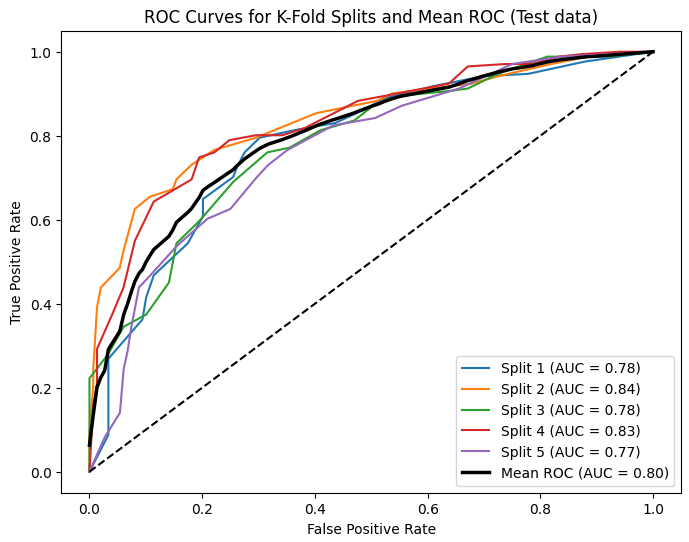
\includegraphics[width=\columnwidth]{plots/dt_wine_ROC_curves.png}
    \caption{ROC Curves for Decision Tree Model on Wine Quality Dataset}
    \label{fig:dt_roc_wine}
  \end{figure}


On Table \ref{tab:dt_wine}, the Decision Tree model's metrics, including an accuracy of 73.8\% and an AUC score of 0.801, highlight its capacity to predict wine quality effectively. These results demonstrate the model's ability to capture nonlinear relationships between features, leveraging key attributes such as "alcohol" and "sulphates" to classify wine quality. The high AUC further supports the model’s strong discrimination between "high" and "low" quality classes, as evident in the ROC curves (Figure \ref{fig:dt_roc_wine}).

Figure \ref{fig:dt_roc_wine} depicts the ROC curves across five cross-validation folds, showcasing a consistent mean AUC of 0.80, with individual folds ranging from 0.77 to 0.84. This stability reflects the model's balance in sensitivity and specificity, maintaining reliable predictions across data splits. The black mean ROC curve, significantly above the random classifier line, underscores the tree's ability to identify predictive patterns. However, the smoothness of the curves suggests that the reliance on discrete thresholds might limit the representation of more complex or subtle feature interactions near decision boundaries. This highlights both the strengths and inherent constraints of the Decision Tree's splitting mechanism.

The focus on "alcohol," "total sulfur dioxide," and "sulphates" in the model is a deliberate selection of features that are not only considered important by the splitting criterion of the Decision Tree but had been previously selected in order to artificially increase the predictive power of the model. Focusing on these main predictors, the Decision Tree is particularly good at leveraging simple, information-packed features to construct clear thresholds of distinction between different levels of wine quality. This is in line with the intrinsic capability of this algorithm to handle large, direct relationships.

Less important features such as "residual sugar" not being part of the dataset upon analysis will result in results that are intrinsically affected by an absence of features that may have more subtle or conditional effects. Refining the feature set also allows the model to focus on the most relevant traits while at the same time reducing the potential for noise or overfitting. With this improvement, the algorithm still relies on single-feature splits and thus might not take into consideration complex relationships among those features that were selected-for instance, how "alcohol" and "sulphates" together may influence wine quality. The results do, however, illustrate that the features chosen provided sufficient information to create strong, interpretable splits within the tree.

The algorithm further showed a precision of 76.5\% and recall of 73.7\%, showing its ability in balancing true positive rates against the reduction of false positives. Such results are due to the tree's ability to readjust its structure according to data while still being bounded by predefined hyperparameters, such as the maximum depth and minimum samples per leaf. Decision Trees fundamentally concentrate on enhancing splits based on predominant patterns present in the data, which may result in robust overall performance; however, this can also lead to sporadic misclassification of outlier cases or minority patterns. It could be that an acceptable recall rate of 73.7\% indicates problems with intersecting feature distributions. For example, "volatile acidity" may have similar ranges for both "high" and "low" quality wines, which would lead to misclassifications. Overlapping boundaries may reduce the ability of the decision tree to easily 'draw a line' around the classes, especially with those wines that fall into more borderline quality categories, such as 5 and 6.

\subsubsection{k-Nearest Neighbors}
\subsubsection{Neural Networks}

\subsection{Mushroom Dataset}
\subsubsection{Logistic Regression}
\subsubsection{Decision Trees}
\subsubsection{k-Nearest Neighbors}
\subsubsection{Neural Networks}

\subsection{General Discussion}

\section{Conclusion}
The conclusion goes here.

\nocite{*}
\def\BibTeX{BibTeX}
\bibliographystyle{IEEEtran}
\bibliography{IEEEabrv,./refs}

\end{document}
